% Options for packages loaded elsewhere
% Options for packages loaded elsewhere
\PassOptionsToPackage{unicode}{hyperref}
\PassOptionsToPackage{hyphens}{url}
%
\documentclass[
  11pt,
  ignorenonframetext,
  aspectratio=169,
  russian,
]{beamer}
\newif\ifbibliography
\usepackage{pgfpages}
\setbeamertemplate{caption}[numbered]
\setbeamertemplate{caption label separator}{: }
\setbeamercolor{caption name}{fg=normal text.fg}
\beamertemplatenavigationsymbolshorizontal
% remove section numbering
\setbeamertemplate{part page}{
  \centering
  \begin{beamercolorbox}[sep=16pt,center]{part title}
    \usebeamerfont{part title}\insertpart\par
  \end{beamercolorbox}
}
\setbeamertemplate{section page}{
  \centering
  \begin{beamercolorbox}[sep=12pt,center]{section title}
    \usebeamerfont{section title}\insertsection\par
  \end{beamercolorbox}
}
\setbeamertemplate{subsection page}{
  \centering
  \begin{beamercolorbox}[sep=8pt,center]{subsection title}
    \usebeamerfont{subsection title}\insertsubsection\par
  \end{beamercolorbox}
}
% Prevent slide breaks in the middle of a paragraph
\widowpenalties 1 10000
\raggedbottom
\AtBeginPart{
  \frame{\partpage}
}
\AtBeginSection{
  \ifbibliography
  \else
    \frame{\sectionpage}
  \fi
}
\AtBeginSubsection{
  \frame{\subsectionpage}
}
\usepackage{iftex}
\ifPDFTeX
  \usepackage[T1]{fontenc}
  \usepackage[utf8]{inputenc}
  \usepackage{textcomp} % provide euro and other symbols
\else % if luatex or xetex
  \usepackage{unicode-math} % this also loads fontspec
  \defaultfontfeatures{Scale=MatchLowercase}
  \defaultfontfeatures[\rmfamily]{Ligatures=TeX,Scale=1}
\fi
\usepackage{lmodern}

\usefonttheme{serif} % use mainfont rather than sansfont for slide text
\ifPDFTeX\else
  % xetex/luatex font selection
  \setmainfont[]{DejaVu Serif}
\fi
% Use upquote if available, for straight quotes in verbatim environments
\IfFileExists{upquote.sty}{\usepackage{upquote}}{}
\IfFileExists{microtype.sty}{% use microtype if available
  \usepackage[]{microtype}
  \UseMicrotypeSet[protrusion]{basicmath} % disable protrusion for tt fonts
}{}

\usepackage{color}
\usepackage{fancyvrb}
\newcommand{\VerbBar}{|}
\newcommand{\VERB}{\Verb[commandchars=\\\{\}]}
\DefineVerbatimEnvironment{Highlighting}{Verbatim}{commandchars=\\\{\}}
% Add ',fontsize=\small' for more characters per line
\usepackage{framed}
\definecolor{shadecolor}{RGB}{241,243,245}
\newenvironment{Shaded}{\begin{snugshade}}{\end{snugshade}}
\newcommand{\AlertTok}[1]{\textcolor[rgb]{0.68,0.00,0.00}{#1}}
\newcommand{\AnnotationTok}[1]{\textcolor[rgb]{0.37,0.37,0.37}{#1}}
\newcommand{\AttributeTok}[1]{\textcolor[rgb]{0.40,0.45,0.13}{#1}}
\newcommand{\BaseNTok}[1]{\textcolor[rgb]{0.68,0.00,0.00}{#1}}
\newcommand{\BuiltInTok}[1]{\textcolor[rgb]{0.00,0.23,0.31}{#1}}
\newcommand{\CharTok}[1]{\textcolor[rgb]{0.13,0.47,0.30}{#1}}
\newcommand{\CommentTok}[1]{\textcolor[rgb]{0.37,0.37,0.37}{#1}}
\newcommand{\CommentVarTok}[1]{\textcolor[rgb]{0.37,0.37,0.37}{\textit{#1}}}
\newcommand{\ConstantTok}[1]{\textcolor[rgb]{0.56,0.35,0.01}{#1}}
\newcommand{\ControlFlowTok}[1]{\textcolor[rgb]{0.00,0.23,0.31}{\textbf{#1}}}
\newcommand{\DataTypeTok}[1]{\textcolor[rgb]{0.68,0.00,0.00}{#1}}
\newcommand{\DecValTok}[1]{\textcolor[rgb]{0.68,0.00,0.00}{#1}}
\newcommand{\DocumentationTok}[1]{\textcolor[rgb]{0.37,0.37,0.37}{\textit{#1}}}
\newcommand{\ErrorTok}[1]{\textcolor[rgb]{0.68,0.00,0.00}{#1}}
\newcommand{\ExtensionTok}[1]{\textcolor[rgb]{0.00,0.23,0.31}{#1}}
\newcommand{\FloatTok}[1]{\textcolor[rgb]{0.68,0.00,0.00}{#1}}
\newcommand{\FunctionTok}[1]{\textcolor[rgb]{0.28,0.35,0.67}{#1}}
\newcommand{\ImportTok}[1]{\textcolor[rgb]{0.00,0.46,0.62}{#1}}
\newcommand{\InformationTok}[1]{\textcolor[rgb]{0.37,0.37,0.37}{#1}}
\newcommand{\KeywordTok}[1]{\textcolor[rgb]{0.00,0.23,0.31}{\textbf{#1}}}
\newcommand{\NormalTok}[1]{\textcolor[rgb]{0.00,0.23,0.31}{#1}}
\newcommand{\OperatorTok}[1]{\textcolor[rgb]{0.37,0.37,0.37}{#1}}
\newcommand{\OtherTok}[1]{\textcolor[rgb]{0.00,0.23,0.31}{#1}}
\newcommand{\PreprocessorTok}[1]{\textcolor[rgb]{0.68,0.00,0.00}{#1}}
\newcommand{\RegionMarkerTok}[1]{\textcolor[rgb]{0.00,0.23,0.31}{#1}}
\newcommand{\SpecialCharTok}[1]{\textcolor[rgb]{0.37,0.37,0.37}{#1}}
\newcommand{\SpecialStringTok}[1]{\textcolor[rgb]{0.13,0.47,0.30}{#1}}
\newcommand{\StringTok}[1]{\textcolor[rgb]{0.13,0.47,0.30}{#1}}
\newcommand{\VariableTok}[1]{\textcolor[rgb]{0.07,0.07,0.07}{#1}}
\newcommand{\VerbatimStringTok}[1]{\textcolor[rgb]{0.13,0.47,0.30}{#1}}
\newcommand{\WarningTok}[1]{\textcolor[rgb]{0.37,0.37,0.37}{\textit{#1}}}

\usepackage{longtable,booktabs,array}
\newcounter{none} % for unnumbered tables
\usepackage{calc} % for calculating minipage widths
\usepackage{caption}
% Make caption package work with longtable
\makeatletter
\def\fnum@table{\tablename~\thetable}
\makeatother
\usepackage{graphicx}
\makeatletter
\newsavebox\pandoc@box
\newcommand*\pandocbounded[1]{% scales image to fit in text height/width
  \sbox\pandoc@box{#1}%
  \Gscale@div\@tempa{\textheight}{\dimexpr\ht\pandoc@box+\dp\pandoc@box\relax}%
  \Gscale@div\@tempb{\linewidth}{\wd\pandoc@box}%
  \ifdim\@tempb\p@<\@tempa\p@\let\@tempa\@tempb\fi% select the smaller of both
  \ifdim\@tempa\p@<\p@\scalebox{\@tempa}{\usebox\pandoc@box}%
  \else\usebox{\pandoc@box}%
  \fi%
}
% Set default figure placement to htbp
\def\fps@figure{htbp}
\makeatother



\ifLuaTeX
\usepackage[bidi=basic,shorthands=off,provide=*]{babel}
\else
\usepackage[bidi=default,shorthands=off,provide=*]{babel}
\fi
\ifPDFTeX
\else
\babelfont{rm}[]{DejaVu Serif}
\fi
\ifLuaTeX
  \usepackage{selnolig} % disable illegal ligatures
\fi


\setlength{\emergencystretch}{3em} % prevent overfull lines

\providecommand{\tightlist}{%
  \setlength{\itemsep}{0pt}\setlength{\parskip}{0pt}}



 

\usepackage[]{csquotes}

\IfFileExists{plex-otf.sty}{
  %% Full TeXlive
  % \usepackage[%
  %   % math,
  %   RM={Scale=0.94},SS={Scale=0.94},SScon={Scale=0.94},TT={Scale=MatchLowercase,FakeStretch=0.9},DefaultFeatures={Ligatures=Common}
  % ]{plex-otf}
}{
  %% TinyTeX
  \usepackage{libertine}
}

%%% Load theme
% https://deic.uab.cat/~iblanes/beamer_gallery/
\IfFileExists{beamerthemegotham.sty}{
  %% Full TeXlive
  \usetheme{gotham}
  \gothamset{
    numbering=totalpagenumber,
    parttocframe default=off,
    sectiontocframe default=off,
    subsectiontocframe default=off,
  }
}{
  %% TinyTeX
  \usetheme{Madrid}
}
\makeatletter
\@ifpackageloaded{caption}{}{\usepackage{caption}}
\AtBeginDocument{%
\ifdefined\contentsname
  \renewcommand*\contentsname{Содержание}
\else
  \newcommand\contentsname{Содержание}
\fi
\ifdefined\listfigurename
  \renewcommand*\listfigurename{Список иллюстраций}
\else
  \newcommand\listfigurename{Список иллюстраций}
\fi
\ifdefined\listtablename
  \renewcommand*\listtablename{Список таблиц}
\else
  \newcommand\listtablename{Список таблиц}
\fi
\ifdefined\figurename
  \renewcommand*\figurename{Рисунок}
\else
  \newcommand\figurename{Рисунок}
\fi
\ifdefined\tablename
  \renewcommand*\tablename{Таблица}
\else
  \newcommand\tablename{Таблица}
\fi
}
\@ifpackageloaded{float}{}{\usepackage{float}}
\floatstyle{ruled}
\@ifundefined{c@chapter}{\newfloat{codelisting}{h}{lop}}{\newfloat{codelisting}{h}{lop}[chapter]}
\floatname{codelisting}{Список}
\newcommand*\listoflistings{\listof{codelisting}{Листинги}}
\makeatother
\makeatletter
\makeatother
\makeatletter
\@ifpackageloaded{caption}{}{\usepackage{caption}}
\@ifpackageloaded{subcaption}{}{\usepackage{subcaption}}
\makeatother

\usepackage{bookmark}
\IfFileExists{xurl.sty}{\usepackage{xurl}}{} % add URL line breaks if available
\urlstyle{same}
\hypersetup{
  pdftitle={Отчет по первому разделу внешнего курса},
  pdfauthor={Лопатченко Полина Андреевна},
  pdflang={ru},
  hidelinks,
  pdfcreator={LaTeX via pandoc}}


\title{\texorpdfstring{Отчет по первому разделу внешнего
курса}{Отчет по первому разделу внешнего курса}}
\subtitle{\texorpdfstring{Введение}{Введение}}
\author{Лопатченко Полина Андреевна}
\date{2026-04-26}

\begin{document}
\frame{\titlepage}

\renewcommand*\contentsname{Содержание}
\begin{frame}[allowframebreaks]
  \frametitle{Содержание}
  \setcounter{tocdepth}{1}
  \tableofcontents
\end{frame}
\setcounter{tocdepth}{1}
\tableofcontents
}

\section{Информация}\label{ux438ux43dux444ux43eux440ux43cux430ux446ux438ux44f}

\begin{frame}{Докладчик}
\protect\phantomsection\label{ux434ux43eux43aux43bux430ux434ux447ux438ux43a}
\begin{columns}[T]
\begin{column}{0.6\linewidth}
\begin{itemize}[<+->]
\tightlist
\item
  Лопатченко Полина Андреевна
\item
  Студент
\item
  НКАбд-04-25
\item
  Российский университет дружбы народов им. П. Лумумбы
\item
  1032253529@rudn.ru
\item
  https://PALopatchenko-lab.github.io/ru/
\end{itemize}
\end{column}

\begin{column}{0.4\linewidth}

\includegraphics[width=0.6\linewidth,height=\textheight,keepaspectratio]{image/я.jpg}
\end{column}
\end{columns}
\end{frame}

\section{Цель и
задачи}\label{ux446ux435ux43bux44c-ux438-ux437ux430ux434ux430ux447ux438}

\begin{frame}{Цель}
\protect\phantomsection\label{ux446ux435ux43bux44c}
Пройти первый этап внешнего курса «Введение в Linux» и закрепить базовые
навыки работы в Linux.
\end{frame}

\begin{frame}{Задачи}
\protect\phantomsection\label{ux437ux430ux434ux430ux447ux438}
\begin{itemize}[<+->]
\tightlist
\item
  изучить общие сведения о курсе и установке Linux;
\item
  освоить базовые команды терминала;
\item
  разобраться со стандартными потоками ввода и вывода;
\item
  изучить основные приёмы скачивания файлов;
\item
  рассмотреть работу с архивами;
\item
  выполнить задания по поиску файлов и текста.
\end{itemize}
\end{frame}

\section{Что такое Linux и зачем нужен
терминал}\label{ux447ux442ux43e-ux442ux430ux43aux43eux435-linux-ux438-ux437ux430ux447ux435ux43c-ux43dux443ux436ux435ux43d-ux442ux435ux440ux43cux438ux43dux430ux43b}

\begin{frame}{Что такое Linux и зачем нужен терминал}
Linux --- это семейство Unix-подобных операционных систем.
\end{frame}

\begin{frame}{Терминал позволяет}
\protect\phantomsection\label{ux442ux435ux440ux43cux438ux43dux430ux43b-ux43fux43eux437ux432ux43eux43bux44fux435ux442}
\begin{itemize}[<+->]
\tightlist
\item
  выполнять команды напрямую;
\item
  управлять файлами и каталогами;
\item
  запускать программы;
\item
  работать со стандартными потоками;
\item
  быстро автоматизировать типовые действия.
\end{itemize}

Именно поэтому в курсе большое внимание уделяется командной строке.
\end{frame}

\section{Что изучалось на первом
этапе}\label{ux447ux442ux43e-ux438ux437ux443ux447ux430ux43bux43eux441ux44c-ux43dux430-ux43fux435ux440ux432ux43eux43c-ux44dux442ux430ux43fux435}

\begin{frame}[fragile]{Что изучалось на первом этапе}
В ходе первого этапа были рассмотрены следующие темы:

\begin{itemize}[<+->]
\tightlist
\item
  общая информация о курсе;
\item
  установка и запуск Linux;
\item
  базовые сведения о пакетах и программах;
\item
  терминал и основные команды;
\item
  ввод, вывод и перенаправление потоков;
\item
  скачивание файлов с помощью \texttt{wget};
\item
  работа с архивами;
\item
  поиск файлов и строк в текстах.
\end{itemize}
\end{frame}

\section{Общая информация о
курсе}\label{ux43eux431ux449ux430ux44f-ux438ux43dux444ux43eux440ux43cux430ux446ux438ux44f-ux43e-ux43aux443ux440ux441ux435}

\begin{frame}{Общая информация о курсе}
На начальном этапе были выполнены вводные задания:

\begin{itemize}[<+->]
\tightlist
\item
  определено название курса;
\item
  изучены правила прохождения курса;
\item
  подтверждён запуск Linux на компьютере.
\end{itemize}

\begin{columns}[T]
\begin{column}{0.5\linewidth}
\begin{figure}[H]

{\centering 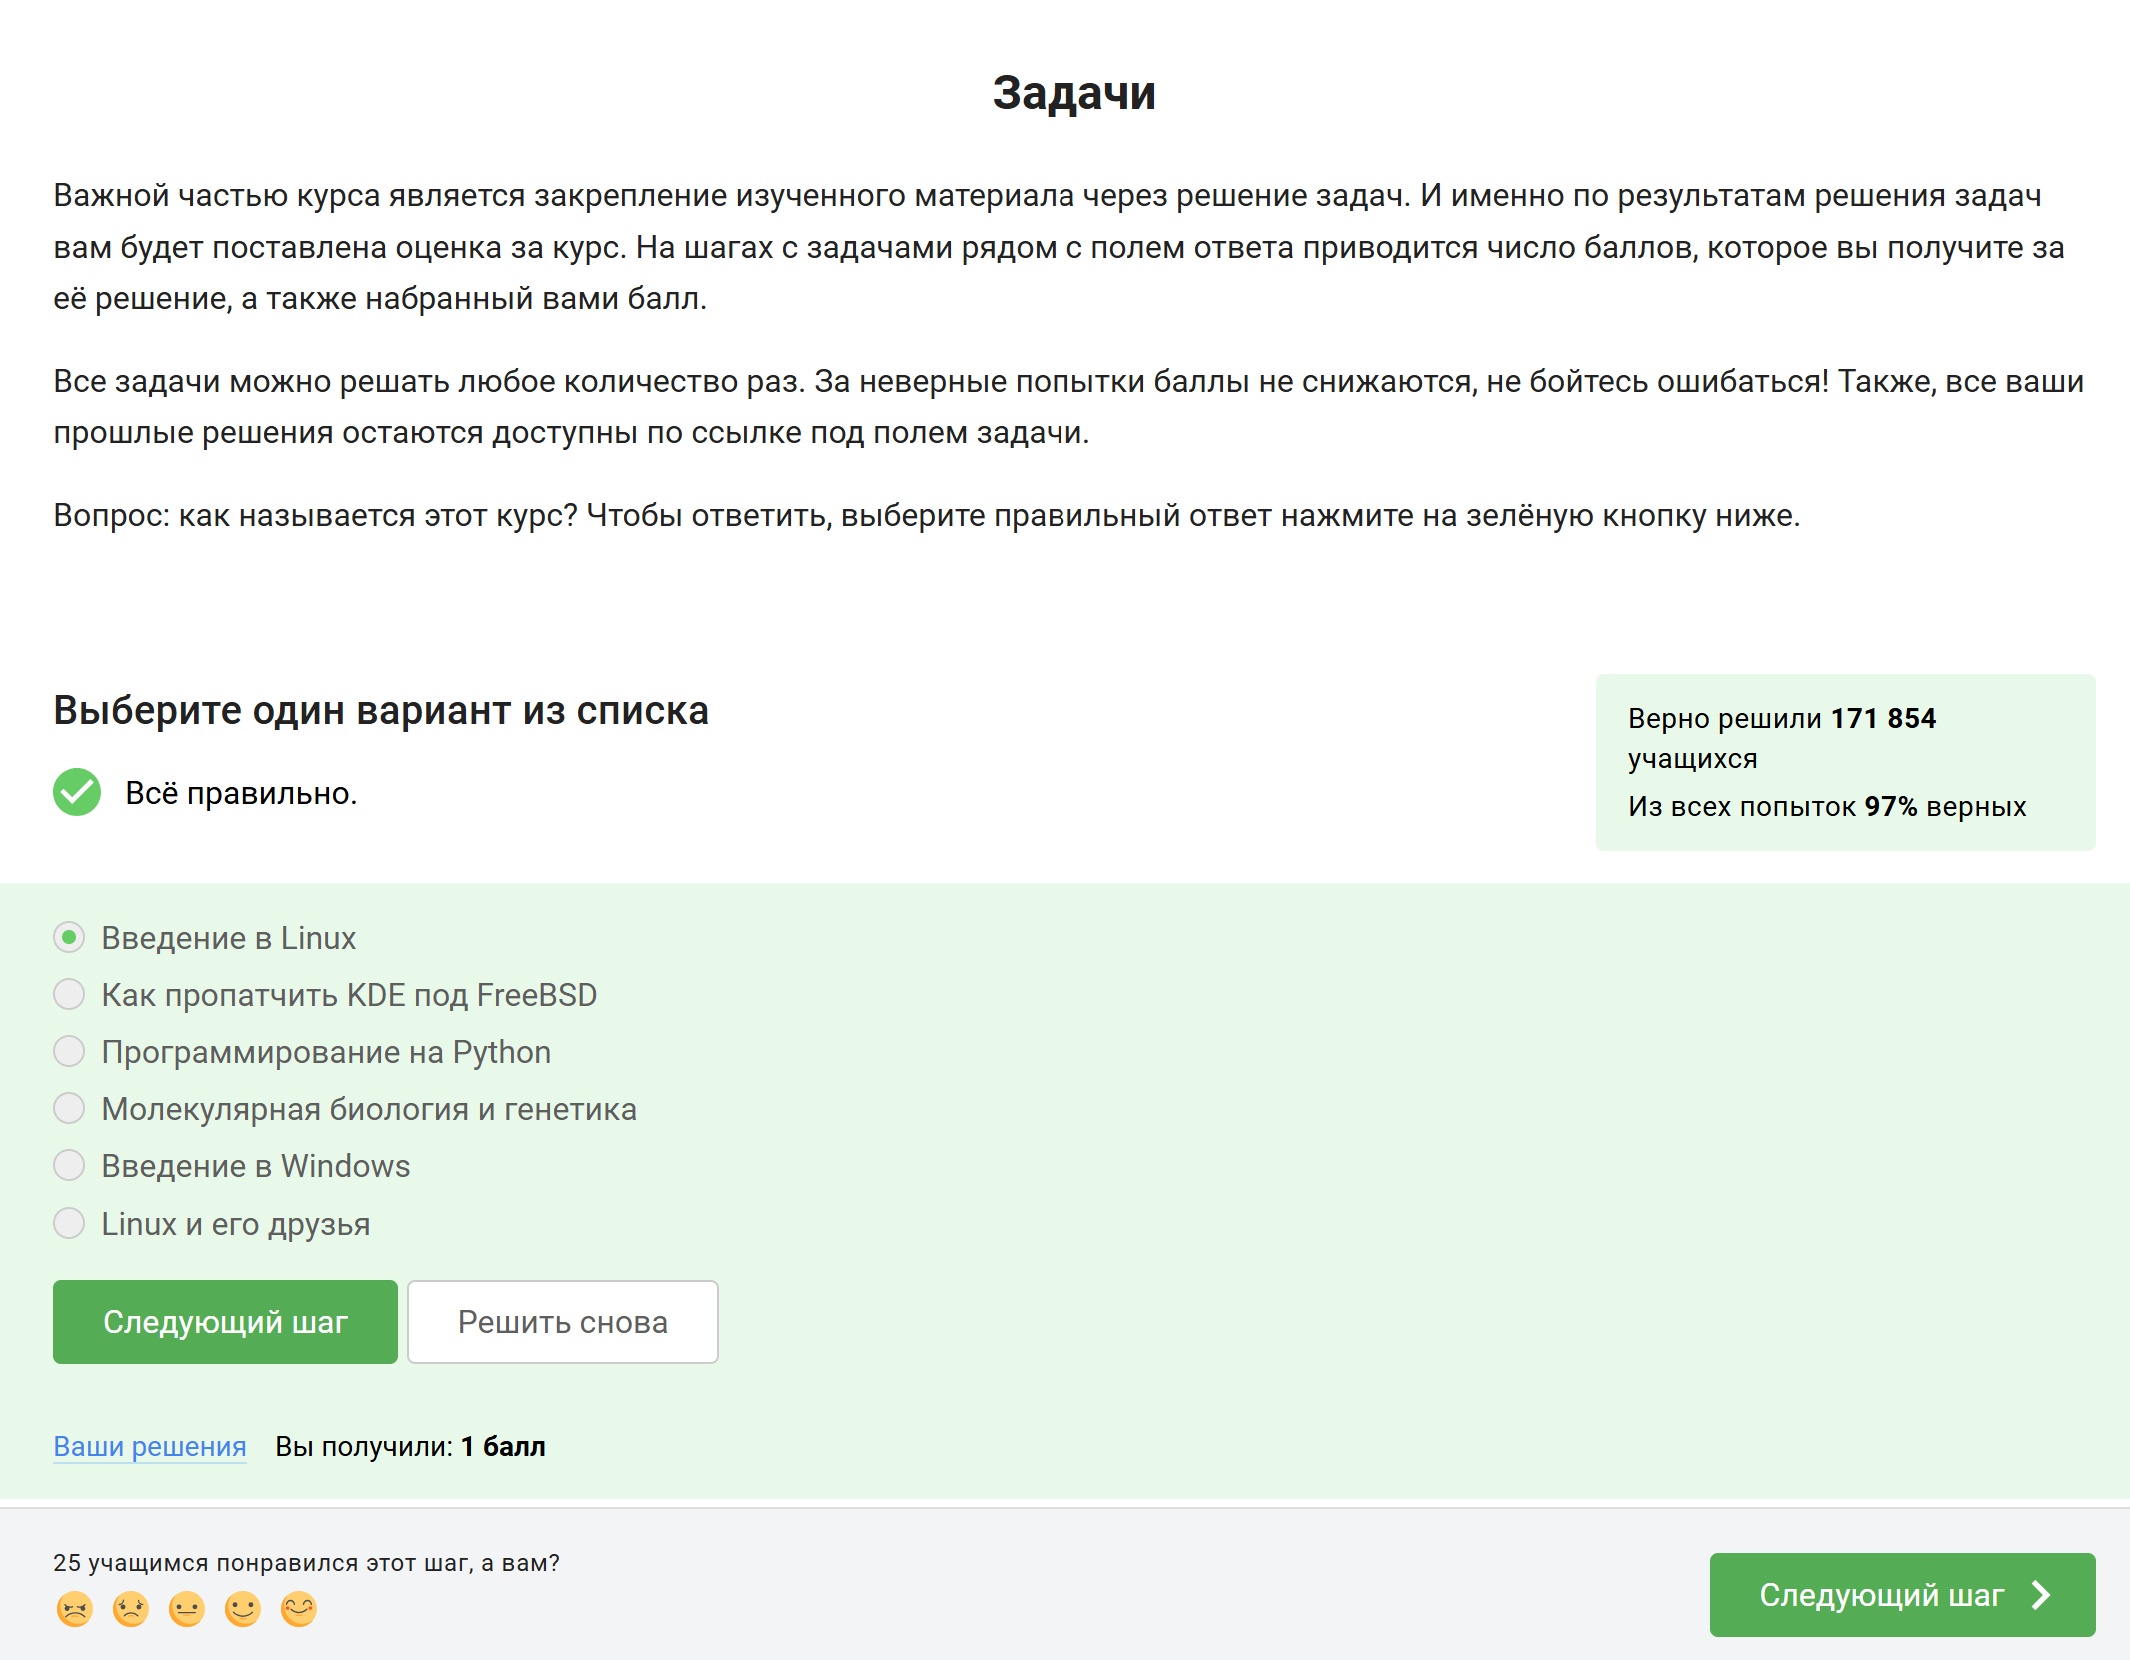
\includegraphics[width=0.8\linewidth,height=\textheight,keepaspectratio]{image/1.png}

}

\caption{Выбор названия курса}

\end{figure}%
\end{column}

\begin{column}{0.5\linewidth}
\begin{figure}[H]

{\centering 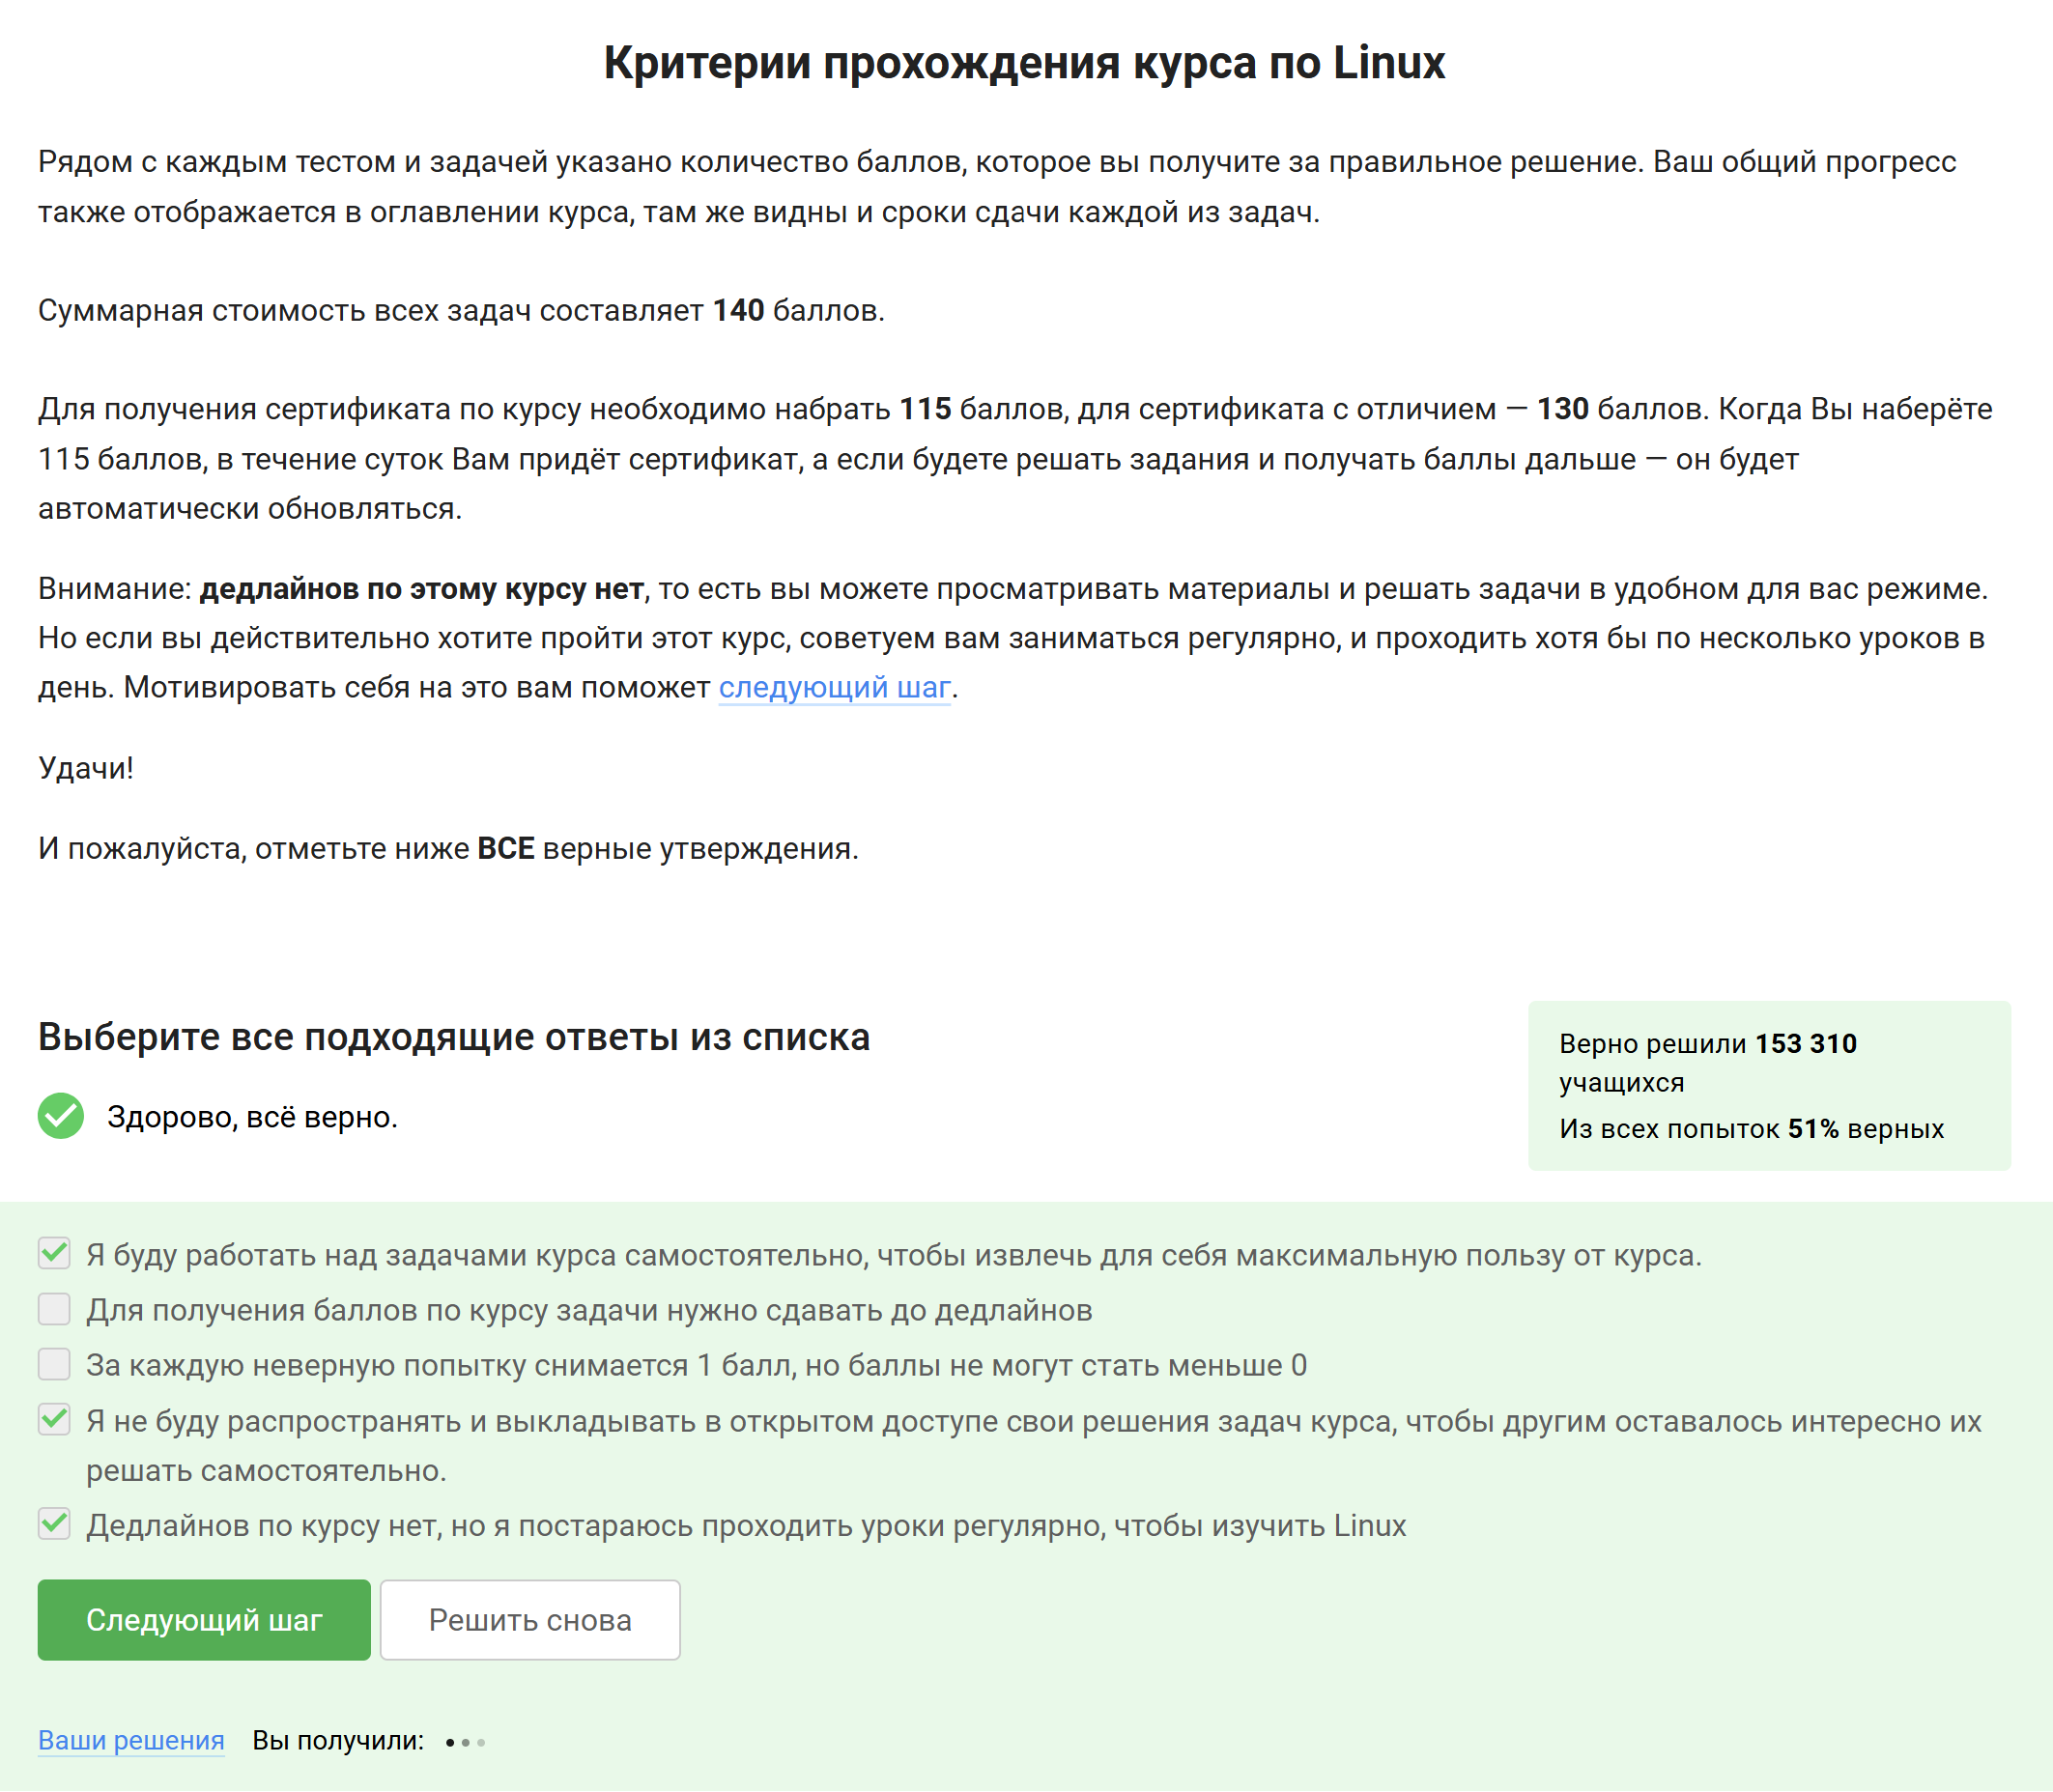
\includegraphics[width=0.8\linewidth,height=\textheight,keepaspectratio]{image/2.png}

}

\caption{Выбор утверждений о прохождении курса}

\end{figure}%
\end{column}
\end{columns}
\end{frame}

\section{Как установить и запустить
Linux}\label{ux43aux430ux43a-ux443ux441ux442ux430ux43dux43eux432ux438ux442ux44c-ux438-ux437ux430ux43fux443ux441ux442ux438ux442ux44c-linux}

\begin{frame}{Как установить и запустить Linux}
Также были рассмотрены базовые вопросы, связанные с установкой Linux и
использованием виртуальной машины.
\end{frame}

\begin{frame}{Было отмечено}
\protect\phantomsection\label{ux431ux44bux43bux43e-ux43eux442ux43cux435ux447ux435ux43dux43e}
\begin{itemize}[<+->]
\tightlist
\item
  какие операционные системы используются обычно;
\item
  что виртуальная машина позволяет запускать одну ОС внутри другой;
\item
  что Linux был успешно запущен на компьютере.
\end{itemize}
\end{frame}

\section{Осваиваем
Linux}\label{ux43eux441ux432ux430ux438ux432ux430ux435ux43c-linux}

\begin{frame}[fragile]{Осваиваем Linux}
На этом этапе были выполнены простые практические задания:

\begin{itemize}[<+->]
\tightlist
\item
  создан текстовый документ в LibreOffice Writer;
\item
  определено расширение пакетов в Ubuntu --- \texttt{deb};
\item
  установлен VLC и найден нужный автор;
\item
  рассмотрены возможности Update Manager.
\end{itemize}
\end{frame}

\section{Пример практического
задания}\label{ux43fux440ux438ux43cux435ux440-ux43fux440ux430ux43aux442ux438ux447ux435ux441ux43aux43eux433ux43e-ux437ux430ux434ux430ux43dux438ux44f}

\begin{frame}[fragile]{Пример практического задания}
Одним из заданий было создание документа со строкой
\texttt{Hello,\ Linux!}, сохранение его в нужном формате и загрузка на
платформу.

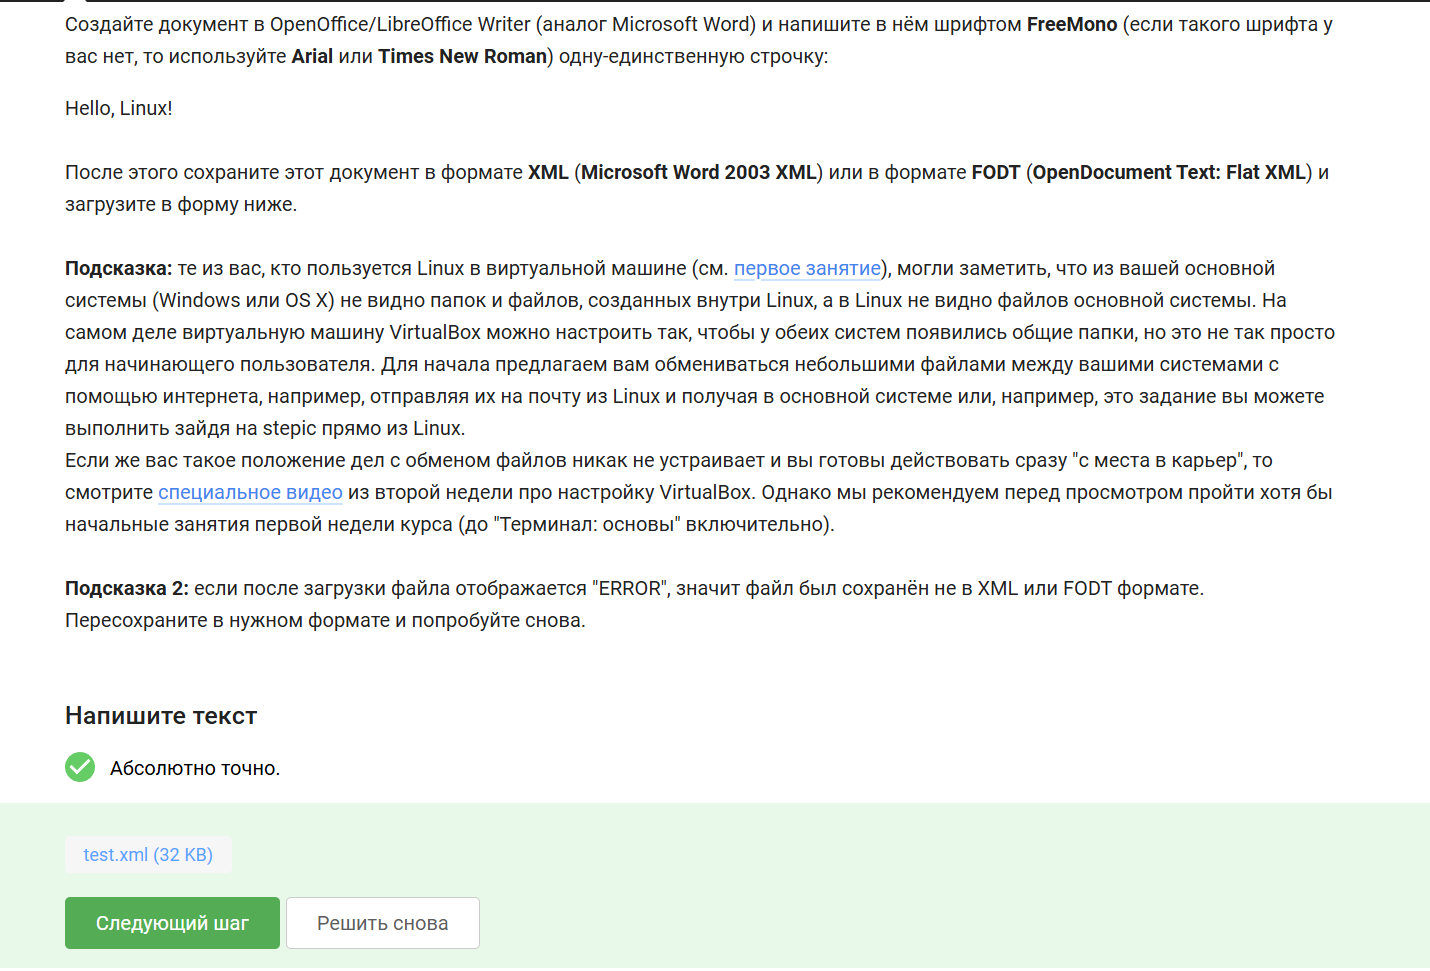
\includegraphics[width=0.65\linewidth,height=\textheight,keepaspectratio]{image/7.png}
\end{frame}

\section{Terminal:
основы}\label{terminal-ux43eux441ux43dux43eux432ux44b}

\begin{frame}[fragile]{Terminal: основы}
В разделе, посвящённом терминалу, были изучены основные понятия и
команды:

\begin{itemize}[<+->]
\tightlist
\item
  \texttt{pwd} --- вывод текущего каталога;
\item
  \texttt{ls} --- просмотр содержимого каталога;
\item
  \texttt{rm\ -r} --- удаление каталогов;
\item
  \texttt{\&}, \texttt{Ctrl+Z}, \texttt{bg} --- работа с фоновыми
  процессами.
\end{itemize}

Также были выполнены задания на понимание путей, опций команд и
поведения программ в терминале.
\end{frame}

\section{Основные идеи раздела
Terminal}\label{ux43eux441ux43dux43eux432ux43dux44bux435-ux438ux434ux435ux438-ux440ux430ux437ux434ux435ux43bux430-terminal}

\begin{frame}[fragile]{Основные идеи раздела Terminal}
В ходе выполнения заданий было установлено, что:

\begin{itemize}[<+->]
\tightlist
\item
  команды Linux чувствительны к регистру;
\item
  один и тот же результат можно получить разными способами;
\item
  длинные и короткие опции команд могут быть эквивалентны;
\item
  относительные и абсолютные пути позволяют обращаться к одним и тем же
  каталогам;
\item
  запуск программы с \texttt{\&} переводит её в фоновый режим.
\end{itemize}
\end{frame}

\section{Пример задания по работе в
терминале}\label{ux43fux440ux438ux43cux435ux440-ux437ux430ux434ux430ux43dux438ux44f-ux43fux43e-ux440ux430ux431ux43eux442ux435-ux432-ux442ux435ux440ux43cux438ux43dux430ux43bux435}

\begin{frame}[fragile]{Пример задания по работе в терминале}
В одном из заданий нужно было найти полную эквивалентную запись команды
\texttt{ls} с длинными опциями.

\begin{Shaded}
\begin{Highlighting}[]
\FunctionTok{ls} \AttributeTok{{-}A} \AttributeTok{{-}{-}human{-}readable} \AttributeTok{{-}l}\NormalTok{ /some/directory}
\end{Highlighting}
\end{Shaded}

эквивалентна:

\begin{Shaded}
\begin{Highlighting}[]
\FunctionTok{ls} \AttributeTok{{-}lAh}\NormalTok{ /some/directory}
\end{Highlighting}
\end{Shaded}

\begin{figure}[H]

{\centering 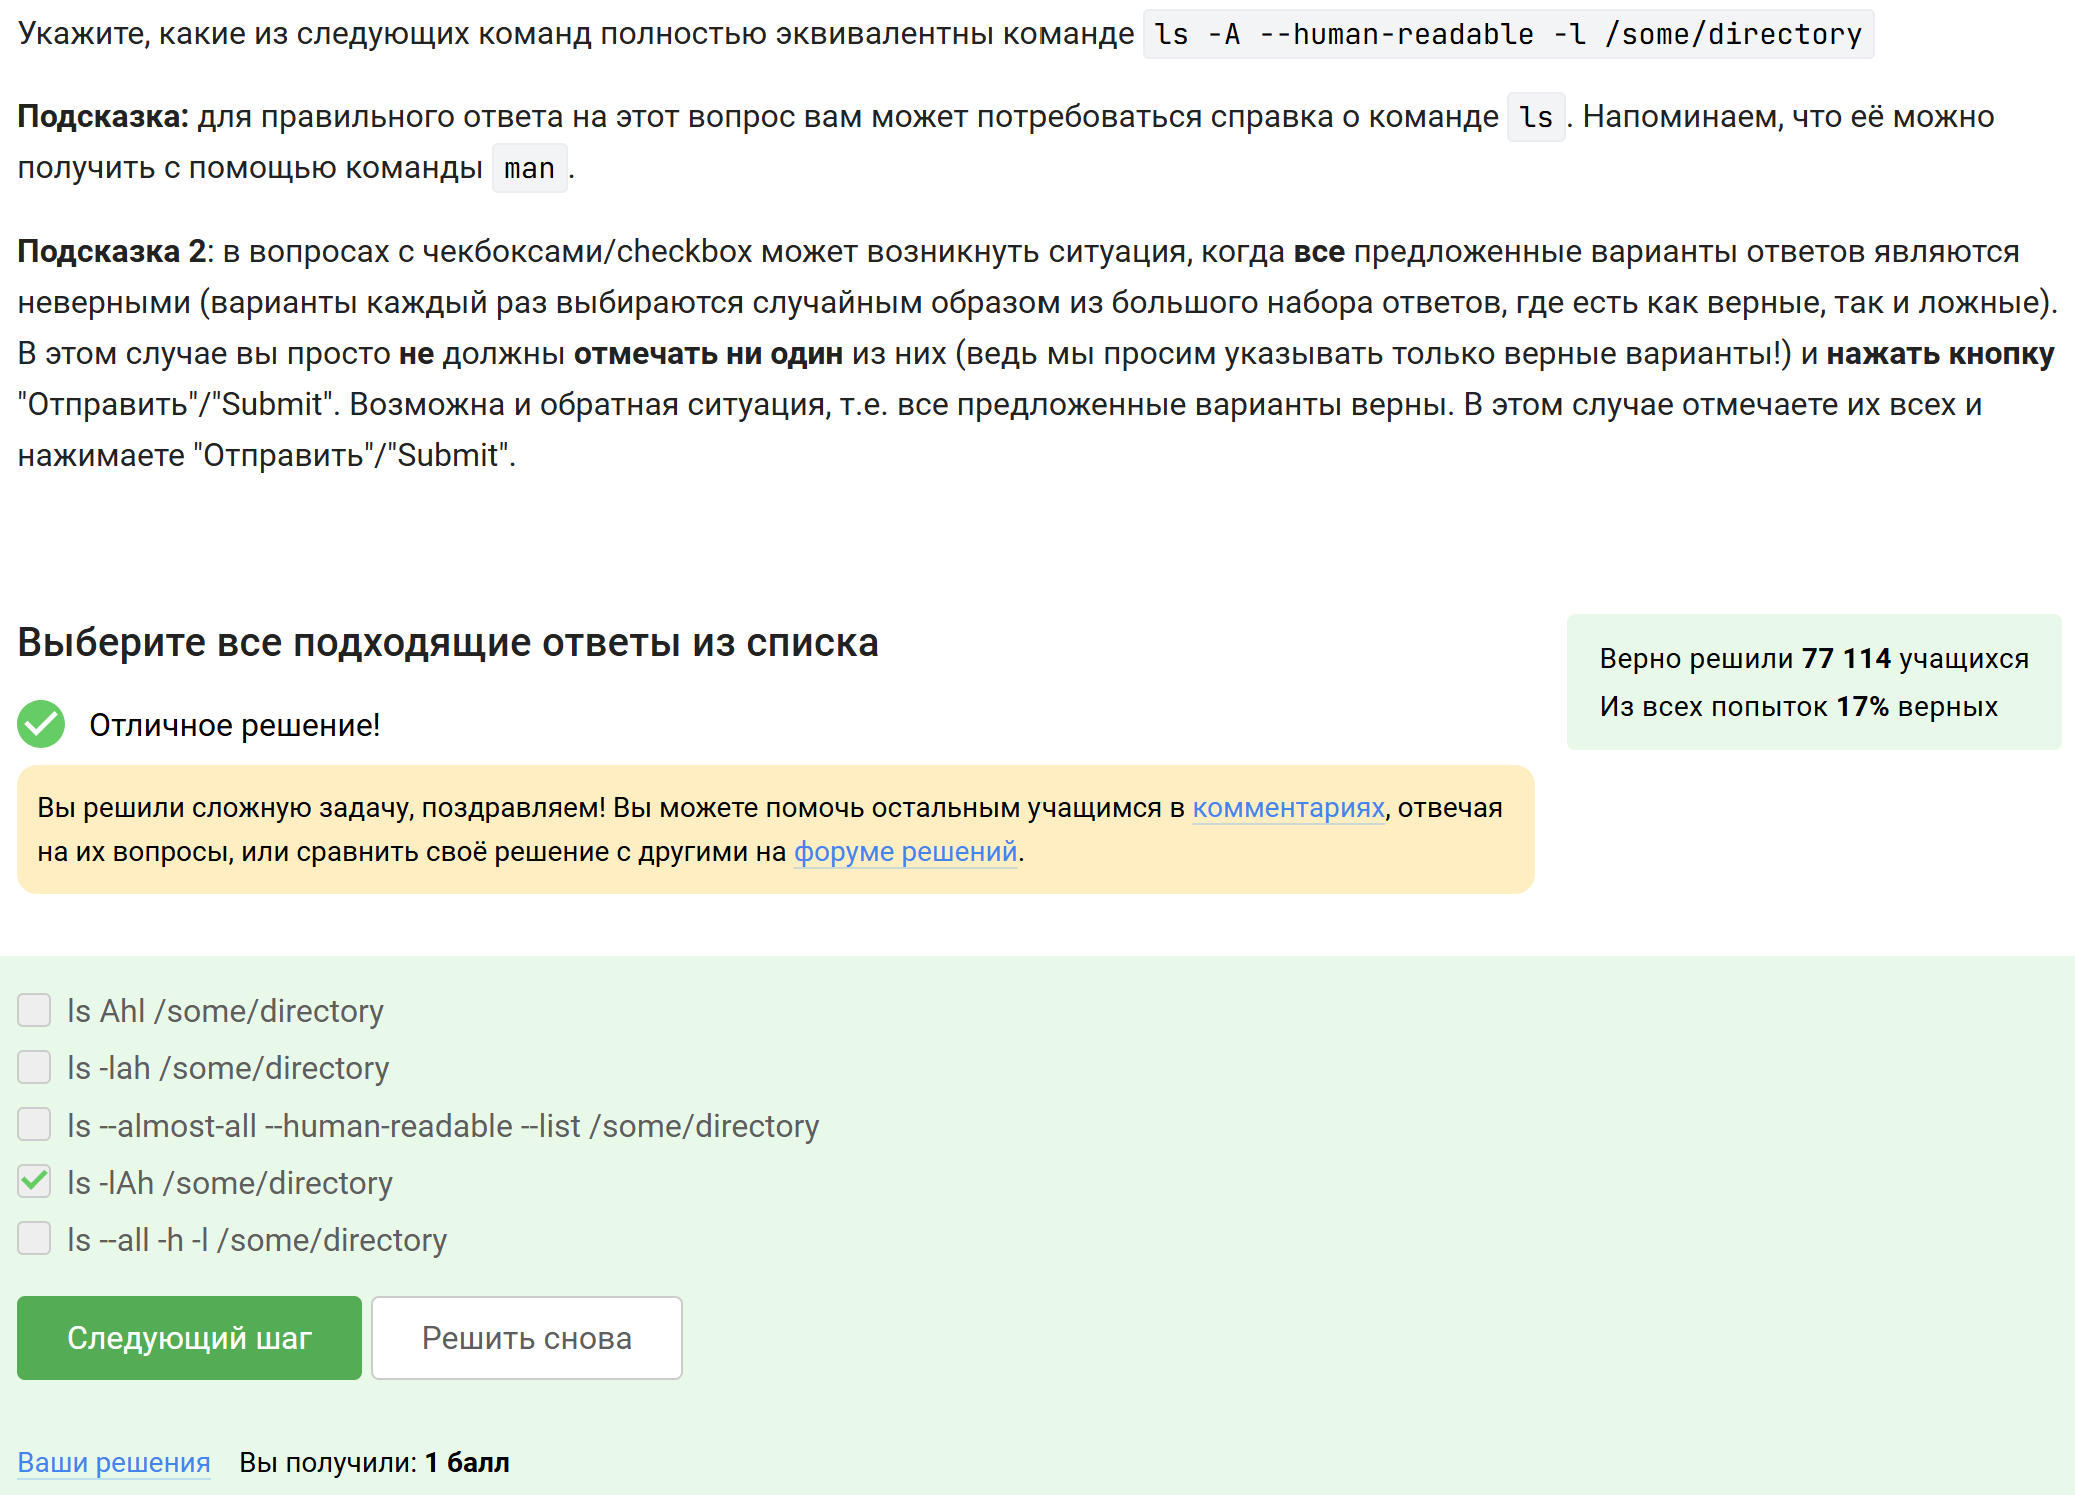
\includegraphics[width=0.45\linewidth,height=\textheight,keepaspectratio]{image/14.png}

}

\caption{Выбор эквивалентной команды ls}

\end{figure}%
\end{frame}

\section{Ввод и
вывод}\label{ux432ux432ux43eux434-ux438-ux432ux44bux432ux43eux434}

\begin{frame}{Ввод и вывод}
Отдельный раздел курса был посвящён стандартным потокам.
\end{frame}

\begin{frame}[fragile]{Были рассмотрены}
\protect\phantomsection\label{ux431ux44bux43bux438-ux440ux430ux441ux441ux43cux43eux442ux440ux435ux43dux44b}
\begin{itemize}[<+->]
\tightlist
\item
  поток обычного вывода \texttt{stdout};
\item
  поток ошибок \texttt{stderr};
\item
  перенаправление в файл с помощью \texttt{\textgreater{}};
\item
  добавление в файл с помощью \texttt{\textgreater{}\textgreater{}};
\item
  перенаправление ошибок через \texttt{2\textgreater{}} и
  \texttt{2\textgreater{}\textgreater{}};
\item
  поведение \texttt{stderr} в конвейере.
\end{itemize}
\end{frame}

\section{Основные выводы по вводу и
выводу}\label{ux43eux441ux43dux43eux432ux43dux44bux435-ux432ux44bux432ux43eux434ux44b-ux43fux43e-ux432ux432ux43eux434ux443-ux438-ux432ux44bux432ux43eux434ux443}

\begin{frame}[fragile]{Основные выводы по вводу и выводу}
В ходе выполнения заданий было установлено, что:

\begin{itemize}[<+->]
\tightlist
\item
  по умолчанию поток ошибок выводится на экран;
\item
  ошибки можно отдельно записывать в файл;
\item
  в конвейере автоматически передаётся только \texttt{stdout};
\item
  \texttt{stderr} остаётся отдельным потоком.
\end{itemize}
\end{frame}

\section{Скачивание файлов из
интернета}\label{ux441ux43aux430ux447ux438ux432ux430ux43dux438ux435-ux444ux430ux439ux43bux43eux432-ux438ux437-ux438ux43dux442ux435ux440ux43dux435ux442ux430}

\begin{frame}[fragile]{Скачивание файлов из интернета}
В этом разделе рассматривалась утилита \texttt{wget}.
\end{frame}

\begin{frame}[fragile]{Были изучены возможности}
\protect\phantomsection\label{ux431ux44bux43bux438-ux438ux437ux443ux447ux435ux43dux44b-ux432ux43eux437ux43cux43eux436ux43dux43eux441ux442ux438}
\begin{itemize}[<+->]
\tightlist
\item
  сохранение файла под нужным именем;
\item
  подавление служебных сообщений через \texttt{-q};
\item
  рекурсивное скачивание;
\item
  фильтрация скачиваемых файлов по расширению.
\end{itemize}

Также были выполнены задания на понимание работы опций:

\begin{itemize}[<+->]
\tightlist
\item
  \texttt{-O};
\item
  \texttt{-P};
\item
  \texttt{-q};
\item
  \texttt{-r};
\item
  \texttt{-l};
\item
  \texttt{-A}.
\end{itemize}
\end{frame}

\section{Работа с
архивами}\label{ux440ux430ux431ux43eux442ux430-ux441-ux430ux440ux445ux438ux432ux430ux43cux438}

\begin{frame}[fragile]{Работа с архивами}
В разделе по архивам рассматривались программы:

\begin{itemize}[<+->]
\tightlist
\item
  \texttt{gzip};
\item
  \texttt{zip};
\item
  \texttt{tar}.
\end{itemize}
\end{frame}

\begin{frame}[fragile]{Было определено}
\protect\phantomsection\label{ux431ux44bux43bux43e-ux43eux43fux440ux435ux434ux435ux43bux435ux43dux43e}
\begin{itemize}[<+->]
\tightlist
\item
  какие программы могут архивировать каталоги;
\item
  какие опции нужны для создания архива \texttt{tar.bz2}.
\end{itemize}

\begin{Shaded}
\begin{Highlighting}[]
\FunctionTok{tar} \AttributeTok{{-}cjf}\NormalTok{ my\_archive.tar.bz2 folder/}
\end{Highlighting}
\end{Shaded}
\end{frame}

\section{Поиск файлов и слов в
файлах}\label{ux43fux43eux438ux441ux43a-ux444ux430ux439ux43bux43eux432-ux438-ux441ux43bux43eux432-ux432-ux444ux430ux439ux43bux430ux445}

\begin{frame}{Поиск файлов и слов в файлах}
Последний раздел был посвящён поиску.
\end{frame}

\begin{frame}[fragile]{Выполненные задания}
\protect\phantomsection\label{ux432ux44bux43fux43eux43bux43dux435ux43dux43dux44bux435-ux437ux430ux434ux430ux43dux438ux44f}
\begin{itemize}[<+->]
\tightlist
\item
  поиск по маскам через \texttt{find};
\item
  поиск строк через \texttt{grep};
\item
  создание файла с результатами;
\item
  использование перенаправления вывода.
\end{itemize}

Это позволило закрепить работу с шаблонами, регистром символов и поиском
текста в наборах файлов.
\end{frame}

\section{Пример задания на поиск
текста}\label{ux43fux440ux438ux43cux435ux440-ux437ux430ux434ux430ux43dux438ux44f-ux43dux430-ux43fux43eux438ux441ux43a-ux442ux435ux43aux441ux442ux430}

\begin{frame}[fragile]{Пример задания на поиск текста}
Одним из практических заданий был поиск всех строк со словом
\texttt{love}.

\begin{columns}[T]
\begin{column}{0.5\linewidth}
\begin{figure}[H]

{\centering 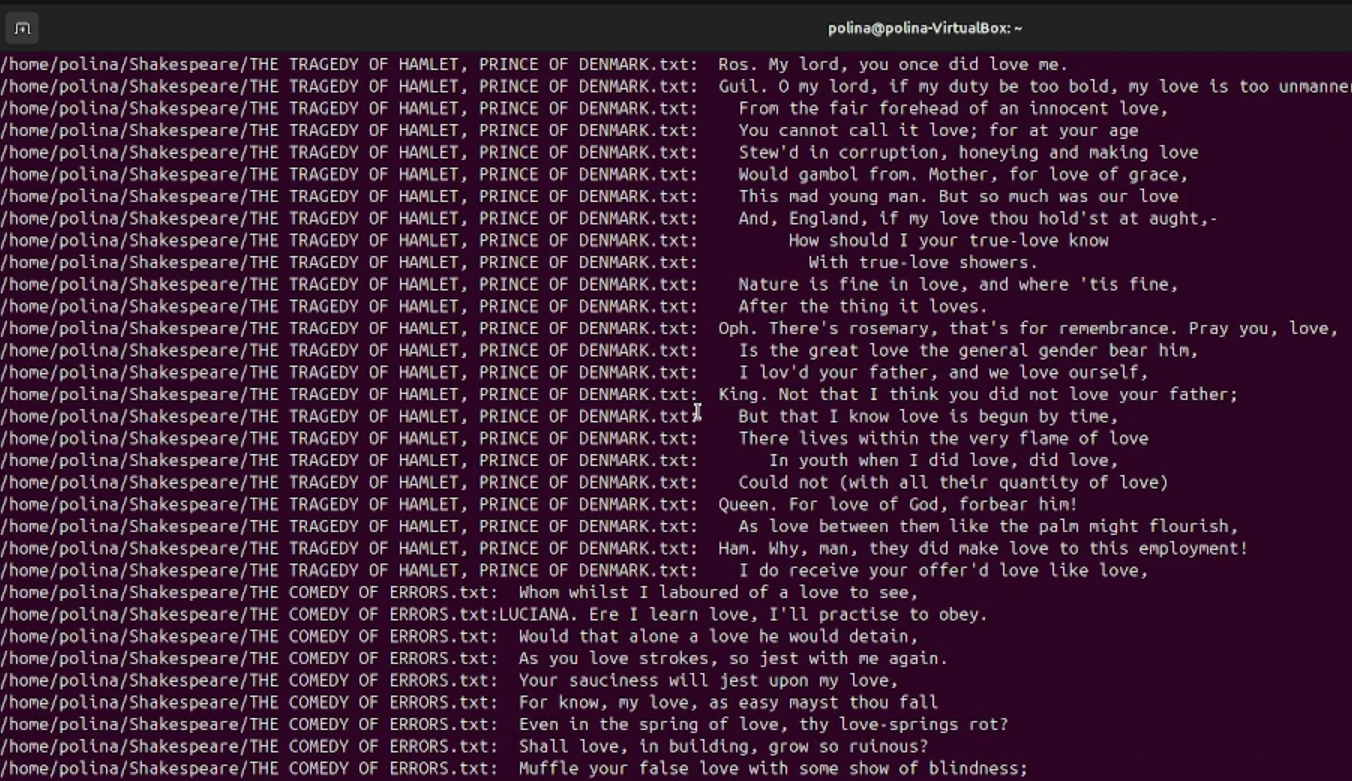
\includegraphics[width=0.9\linewidth,height=\textheight,keepaspectratio]{image/32.png}

}

\caption{Поиск строк со словом love}

\end{figure}%
\end{column}

\begin{column}{0.5\linewidth}
\begin{figure}[H]

{\centering 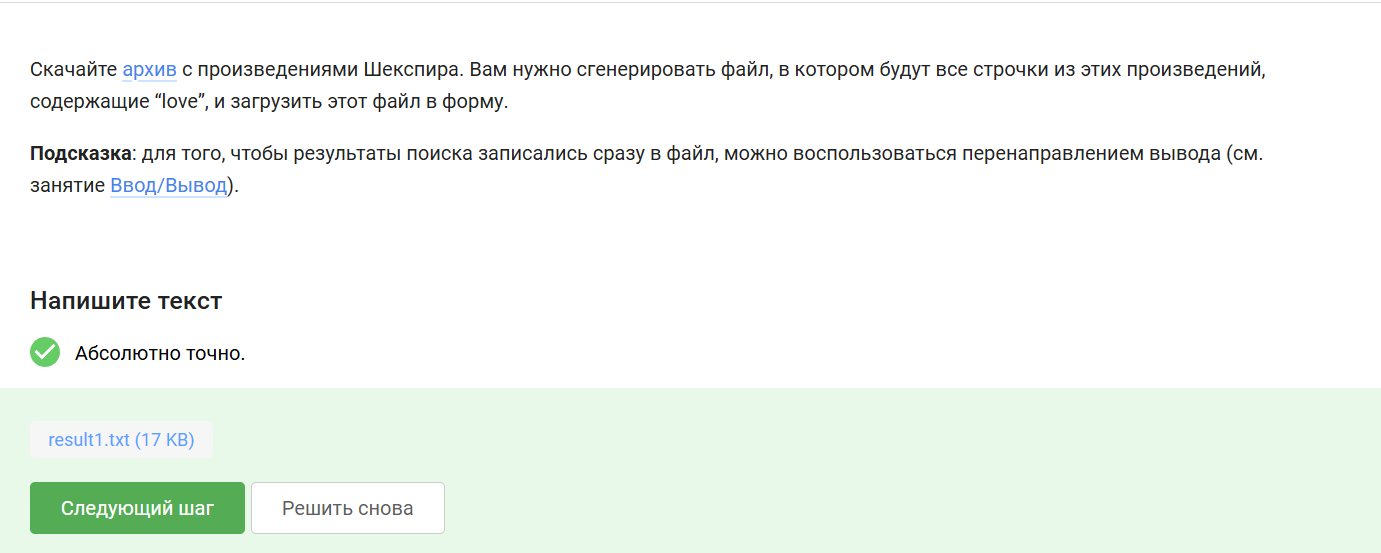
\includegraphics[width=0.9\linewidth,height=\textheight,keepaspectratio]{image/33.png}

}

\caption{Загрузка файла answer.txt}

\end{figure}%
\end{column}
\end{columns}
\end{frame}

\section{Результаты прохождения
этапа}\label{ux440ux435ux437ux443ux43bux44cux442ux430ux442ux44b-ux43fux440ux43eux445ux43eux436ux434ux435ux43dux438ux44f-ux44dux442ux430ux43fux430}

\begin{frame}{Результаты прохождения этапа}
По итогам выполнения первого этапа были закреплены следующие навыки:

\begin{itemize}[<+->]
\tightlist
\item
  работа с базовыми командами Linux;
\item
  понимание относительных и абсолютных путей;
\item
  использование стандартных потоков и перенаправления;
\item
  скачивание файлов из интернета;
\item
  работа с архивами;
\item
  поиск файлов и строк в текстовых файлах.
\end{itemize}

Таким образом, первый этап курса сформировал основу для дальнейшего
изучения Linux.
\end{frame}

\section{Выводы}\label{ux432ux44bux432ux43eux434ux44b}

\begin{frame}{Выводы}
В ходе выполнения работы был пройден первый этап внешнего курса
«Введение в Linux».

В процессе прохождения этапа были изучены базовые теоретические сведения
и выполнены практические задания по работе с терминалом, вводом и
выводом, скачиванием файлов, архивами и поиском текста.
\end{frame}




\end{document}
